\section{Matchings}
\authors{Petula Diemke und Theresa Schwarz}

\begin{figure}[ht]
\centering
   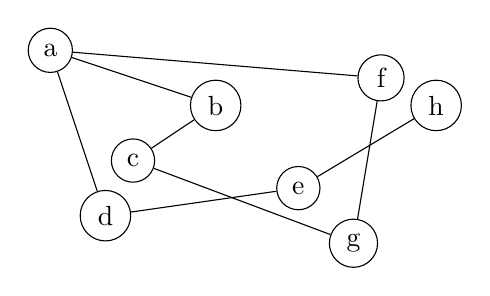
\begin{tikzpicture}[scale=0.7]
   \node[draw,circle](a) at (0,3.5){a};
   \node[draw,circle](b) at (3,2.5){b};
   \node[draw,circle](c) at (1.5,1.5){c};
   \node[draw,circle](d) at (1,0.5){d};
   \node[draw,circle](e) at (4.5,1){e};
   \node[draw,circle](f) at (6,3){f};
   \node[draw,circle](g) at (5.5,0){g};
   \node[draw,circle](h) at (7,2.5){h};
   \draw (a)--(b);
   \draw (a)--(f);
   \draw (a)--(d);
   \draw (c)--(b);
   \draw (c)--(g);
   \draw (d)--(e);
   \draw (g)--(f);
   \draw (e)--(h);
   \end{tikzpicture}
\caption{Graph $H$}
\label{nomatch}
\end{figure}

\begin{figure}[ht]
\centering
   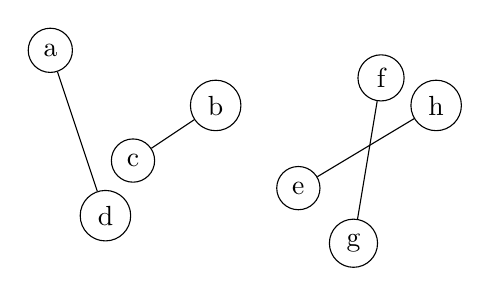
\begin{tikzpicture}[scale=0.7]
   \node[draw,circle](a) at (0,3.5){a};
   \node[draw,circle](b) at (3,2.5){b};
   \node[draw,circle](c) at (1.5,1.5){c};
   \node[draw,circle](d) at (1,0.5){d};
   \node[draw,circle](e) at (4.5,1){e};
   \node[draw,circle](f) at (6,3){f};
   \node[draw,circle](g) at (5.5,0){g};
   \node[draw,circle](h) at (7,2.5){h};
   \draw (a)--(d);
   \draw (c)--(b);
   \draw (g)--(f);
   \draw (e)--(h);
   \end{tikzpicture}
\caption{Matching $M_{1}$ in Graph $H$}
\label{kadimatch}

\end{figure}

\subsection{Was ist ein Matching?}
Ein Matching oder eine Paarung liegt vor, wenn Knoten eines Graphen jeweils paarweise anderen Knoten des Graphen zugeordnet werden. Es können jeweils nur zwei Knoten über eine schon im Graphen vorhandene Kante miteinander gematcht werden.
\begin{df}
Ein \wichtig{Matching} ist eine Untermenge $M$ der Kantenmenge $E$, sodass für alle $e, e' \in M$ mit $e \neq e'$ gilt: $e \cap e' = \emptyset$.
\end{df}
\noindent Das heißt, dass jeder Knoten maximal in einer Kante der Kantenmenge $M$ vorhanden ist. Somit hat jeder Knoten im Matching $M$ höchstens einen Partner.

\subsection{Eigenschaften von Matchings}
Es gibt verschiedene Möglichkeiten ein Matching $M$ in einem Graphen $G$ zu bilden. Gibt es keine Möglichkeit $M$ noch Kanten hinzuzufügen, wird das Matching als maximal bezeichnet. Es werden zwei Arten von maximalen Matchings unterschieden. 

\begin{df}
Ein Matching $M$ heißt \wichtig{kardinalitätsmaximal}, wenn es kein Matching $M'$ gibt, sodass $|M'| > |M|$.
\end{df}

\noindent Diese Definition besagt, dass im Graph $G$ existiert anderes Matching $M'$ existiert, welches mehr Knoten verbindet und somit mehr Kanten als ein kardinalitätsmaximales Matching $M$ besitzt.
Das Matching $M_{1}$ (Abb. \ref{kadimatch}) ist zum Beispiel ein kardinalitätsmaximales Matching in Graph $H$.
\\
\\ Die zweite Möglichkeit eines maximalen Matchings ist ein inklusionsmaximales Matching $M$. Liegt dieses vor, kann einem Matching $M$ in Graph $G$ keine Kante mehr hinzugefügt werden, allerdings muss dieses nicht insgesamt in $G$ das Matching mit der größten Kantenanzahl sein. 

\begin{df}
Ein Matching $M$ heißt \wichtig{inklusionsmaximal}, wenn kein Matching $M'$ existiert, sodass $M \  \subsetneq\ M'$.
\end{df}

\begin{figure}[ht]
\centering
   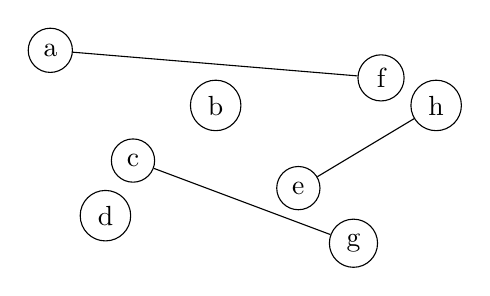
\begin{tikzpicture}[scale=0.7]
   \node[draw,circle](a) at (0,3.5){a};
   \node[draw,circle](b) at (3,2.5){b};
   \node[draw,circle](c) at (1.5,1.5){c};
   \node[draw,circle](d) at (1,0.5){d};
   \node[draw,circle](e) at (4.5,1){e};
   \node[draw,circle](f) at (6,3){f};
   \node[draw,circle](g) at (5.5,0){g};
   \node[draw,circle](h) at (7,2.5){h};
   \draw (a)--(f);
   \draw (c)--(g);
   \draw (e)--(h);
   \end{tikzpicture}
\caption{Matching $M_{2}$ in Graph $H$}
\label{inklumatch}
\end{figure}

\noindent Das Matching $M_{2}$ (Abb. \ref{inklumatch}) ist ein Beispiel für ein inklusionsmaximales Matching in Graph $H$. Bei dieser Konstellation sind keine weitere Verbindungen zwischen Knoten möglich, es gibt in $H$ aber ein anderes Matching $M_{1}$, welches mehr Kanten enthält (Abb. \ref{kadimatch}). Somit ist $M_{2}$ nicht kardinalitätsmaximal.
\\ \noindent \phantom{A}
\\ Ist jeder Knoten in $M$ enthalten, wird das Matching als perfekt bezeichnet. Da jeweils zwei Knoten durch eine Kante aus $M$ verbunden sind, ist die Anzahl der Kanten in $M$ genau die Hälfte der Anzahl der Knoten. Das Matching $M_{1}$ aus Abb. \ref{kadimatch} ist ein Beispiel für ein perfektes Matching. 

\begin{df}
Ein Matching $M$ heißt \wichtig{perfekt}, wenn $|M| = \frac{1}{2} |V|$.
\end{df}

\noindent Wenn ein Graph $G$ eine ungerade Anzahl von Knoten besitzt, dann gibt es kein perfektes Matching, da immer ein Knoten existiert, der nicht mit einem anderen Knoten gematcht ist. Sind aber ansonsten alle Knoten gepaart, dann wird dieses Matching als fast-perfekt bezeichnet. Somit entspricht die Anzahl der Kanten in $M$ der Hälfte der um eins reduzierten Knotenanzahl.

\begin{df}
Ein Matching $M$ heißt \wichtig{fast-perfekt}, wenn $|M| = \frac{1}{2} (|V| - 1)$.
\end{df}

\subsection{Stabiles Matching}
Für den weiteren Verlauf des Kapitels wird angenommen, dass jeder Graph $G$ ein bipartiter Graph ist und jeder Knoten in diesem Graphen eine Präferenzliste hat.

\begin{table}[ht]
\centering
$X=\{1,2,3,4\}$ \ \ \ \ \ \ \ \ \ $Y=\{A,B,C,D\}$
\\ \phantom{A}
$1 \ \ - \ \ A \ \ B \ \ C \ \ D \ \ \ \ \ \ A \ \ - \ \ 4 \ \ 2 \ \ 1 \ \ 3$
\\ $2 \ \ - \ \ D \ \ B \ \ A \ \ C \ \ \ \ \ \ B \ \ - \ \ 3 \ \ 1 \ \ 4 \ \ 2$
\\ $3 \ \ - \ \ B \ \ A \ \ C \ \ D \ \ \ \ \ \ C \ \ - \ \ 1 \ \ 3 \ \ 4 \ \ 2$
\\ $4 \ \ - \ \ D \ \ A \ \ B \ \ C \ \ \ \ \ \ D \ \ - \ \ 1 \ \ 4 \ \ 2 \ \ 3$

\caption{Knoten in Menge $X$ und $Y$ mit  Präferenzliste}
\label{biparprae}
\end{table} 

\phantom{A}
\noindent In einem \wichtig{bipartiten Graphen} ist eine Einteilung der Knoten in zwei Mengen $X$ und $Y$ möglich, sodass innerhalb einer jeden Menge die Knoten nicht miteinander verbunden sind. Die einzigen möglichen Kanten existieren zwischen zwei Knoten unterschiedlicher Mengen. 
\\ Eine \wichtig{Präferenzliste} ist eine Liste eines Knoten einer Menge, in der alle Knoten der anderen Menge vorhanden und nach Präferenz geordnet sind. 
\\ In Tab. \ref{biparprae} ist beispielsweise eine konkrete Instanz für einen bipartiten Graphen $G$ mit den Knotenmengen $X=\{1,2,3,4\}$ und $Y=\{A,B,C,D\}$ mit den jeweiligen Präferenzlisten abgebildet.
\\ \phantom{es}
\\ Ein Matching $M$ in einem bipartiten Graphen $G$ besteht immer aus Kanten zwischen jeweils einem Knoten der einen und einem Knoten der anderen Menge (welche in dieser Betrachtung beide aus der gleichen Anzahl Knoten bestehen). In einem bipartiten Graphen $G$ mit Präferenzliste der Knoten wird meist versucht, ein stabiles Matching $M$ zu erstellen. 

\begin{df}
Ein Matching $M$ heißt \wichtig{stabil}, wenn für jedes Paar $(x, y)$ mit $x \in X$, $y \in Y$ und $\{x, y\} \notin M$ gilt, dass
\\ x seinen Partner gegenüber y präferiert oder 
\\ y seinen Partner gegenüber x präferiert.
\end{df}

\noindent $x$ und $y$ sind Knoten unterschiedlicher Mengen, die nicht miteinander gematcht sind. Bevorzugt $x$ seinen derzeitigen Partner gegenüber $y$ oder bevorzugt $y$ seinen derzeitigen Partner gegenüber $x$, dann ist das Matching stabil, da mindestens einer von $x$ oder $y$ nicht von seinem derzeitigen Partner getrennt und miteinander gematcht werden wollen würde. Wären sie gegenseitig weiter vorn auf ihren Präferenzlisten, würden $x$ und $y$ präferieren, miteinander gematcht zu werden und das momentane Matching $M$ wäre nicht stabil.

\subsection{Ermitteln eines stabilen Matchings}
Für das Ermitteln eines stabilen Matchings $M$ eines bipartiten Graphen $G$ gibt es verschiedene Algorithmen. Der derzeit Beste ist der \wichtig{Gale-Shapely-Algorithmus}.
\begin{enumerate}
\item Alle $x \in X$ stellen Antrag an präferiertes $y \in Y$.
\item Jedes $y \in Y$, das Antrag erhalten hat, akzeptiert den von sich selbst bevorzugten.
\item Nicht-gematchte $x \in X$ stellen Antrag an nächstbestes $y \in Y$.
\\ \ \ \ \ \ Kehre zu Schritt 2 zurück.
\item Wenn alle $x \in X$ gematcht ist der Algorithmus zu Ende.
\end{enumerate}

\noindent Ein bekanntes Beispiel für ein stabiles-Matching-Problem ist das Heiratsproblem. Es gibt eine bestimmte Anzahl Herren und genauso viele Damen, die sich verloben möchten. Nun hat jede der Damen eine Präferenzliste mit der Reihenfolge, in der sie die Herren bevorzugen. Die Herren haben auch jeweils eine Präferenzliste, welche widerum angibt, welche Damen von welchem Herren präferiert werden. Jetzt wird ein stabiles Matching $M$ gesucht.
\\ \phantom{a}
\\ Als Beispiel wird Tab. \ref{biparprae} betrachtet. 1, 2, 3 und 4 sind die Knoten, die die Herren darstellen; A, B, C und D sind die Knoten, die die Damen repräsentieren. Die Herren machen Anträge an die Damen in der Reihenfolge ihrer Präferenzliste, welche in der Abbildung als Aufzählung (der Knoten der anderen Menge) hinter den Knoten dargestellt ist.
\\ Wird zu diesem Beispiel der Gale-Shapely-Algorithmus ausgeführt, dann geschieht folgendes
\\ \phantom{A}
\\ 1 macht A einen Antrag
\\ 2 macht D einen Antrag
\\ 3 macht B einen Antrag
\\ 4 macht D einen Antrag
\\ \phantom{esss} A nimmt Antrag von 1 an
\\ \phantom{esss} B nimmt Antrag von 3 an
\\ \phantom{esss} D nimmt Antrag von 4 an, da 4 präferierter
\\ 2 macht B einen Antrag
\\ \phantom{esss} B lehnt 2 ab, da 3 präferierter
\\ 2 macht A einen Antrag
\\ \phantom{esss} A nimmt Antrag von 2 an, da 2 präferierter
\\ 1 macht B einen Antrag
\\ \phantom{esss} B lehnt Antrag von 1 ab, da 3 präferierter
\\ 1 macht C einen Antrag
\\ \phantom{esss} C nimmt Antrag von 1 an
\\ \ \ \ \ \ $\rightarrow$ stabiles Matching

\begin{table}[ht]
\centering
$X$ \ \ \ \ \ \ \ \ \ \ \ \ \ \ \ \ \ \ \ \ \ \ \ \ \ \ \ \ \ $Y$
$1 \ \ - \ \ A \ \ B \ \ \wichtig{\underline{C}} \ \ D \ \ \ \ \ \ \ \ A \ \ - \ \ 4 \ \ \wichtig{\underline{2}} \ \ 1 \ \ 3$
\\ $2 \ \ - \ \ D \ \ B \ \ \wichtig{\underline{A}} \ \ C \ \ \ \ \ \ \ \ B \ \ - \ \ \wichtig{\underline{3}} \ \ 1 \ \ 4 \ \ 2$
\\ $3 \ \ - \ \ \wichtig{\underline{B}} \ \ A \ \ C \ \ D \ \ \ \ \ \ \ \ C \ \ - \ \ \wichtig{\underline{1}} \ \ 3 \ \ 4 \ \ 2$
\\ $4 \ \ - \ \ \wichtig{\underline{D}} \ \ A \ \ B \ \ C \ \ \ \ \ \ \ \ D \ \ - \ \ 1 \ \ \wichtig{\underline{4}} \ \ 2 \ \ 3$
\caption{Knoten mit \wichtig{\underline{stabilem Matching $M$}}}
\label{bimat}
\end{table} 

\noindent Das vom Gale-Shapely-Algorithmus ausgegebene Matching $M$ ist immer stabil: Angenommen Herr $x$ präferiert Dame $y$ gegenüber seiner aktuellen Partnerin, dann hätte er $y$ irgenwann einen Antrag gemacht. Da sich im Laufe des Algorithmus die Damen dauerhaft verbessern, muss der Herr $x$ weiter hinten auf ihrer Präferenzliste stehen. Ansonsten hätte sie den Antrag angenommen und es käme gar nicht erst zu einem instabilen Matching. Auch bei den Damen besteht nicht die Chance, dass eine von ihnen einen anderen Herren bevorzugt, welcher lieber ihr den Antrag gestellt hätte als seiner derzeitigen Partnerin.